\section{Moment Realizability for the Fermionic Two-Moment Model}
\label{sec:realizability}

Our goal is to simulate a gas of massless fermions (i.e., classical neutrinos) and study their interactions with matter.  
The principal objective is to obtain the fermionic distribution function $f$ (or moments of $f$ as in the two-moment model employed here).  
The Pauli exclusion principle requires the distribution function to satisfy the condition $0 \le f \le 1$, which puts restrictions on the admissible values for the moments of $f$.  
In this paper, we seek to design a numerical method for solving the system of moment equations given by Eq.~\eqref{eq:momentEquations}, which preserves realizability of the moments; i.e., the moments evolve within the set of admissible values as dictated by Pauli's exclusion principle.  
(Since we only concern with the angular dependence of $f$ in this section, we simplify the notation by suppressing the $\vect{z}$ and $t$ dependence and write $f(\omegaNu,\vect{z},t)=f(\omegaNu)$.)  

We begin with the following definition of moment realizability.  
\begin{define}
  The moments $\vect{\cM}=\big(\cJ,\vect{\cH}\big)^{T}$ are realizable if they can be obtained from a distribution function satisfying $0\le f(\omegaNu) \le 1~\forall~\omegaNu\in\bbS^{2}$.
\end{define}

Obviously, realizable moments must satisfy the bounds imposed by $f$.  
We proceed by stating the bounds on the moments by restating (with slightly modified proof) results from Theorem~7.1 in \cite{banachLarecki_2017a} in the following Lemma.  
\begin{lemma}
  Let the distribution function be bounded by $0\le f(\omegaNu) \le1~\forall~\omegaNu\in\bbS^{2}$.  
  Then the moments $\vect{\cM}=(\cJ,\vect{\cH})^{T}$, defined as in Eq.~\eqref{eq:angularMoments}, satisfy $0\le\cJ\le1$ and $\big(1-\cJ\big)\,\cJ-|\vect{\cH}|\ge0$. 
  \label{lem:MomentRealizable} 
\end{lemma}
\begin{proof}
  First, let $\mu=\cos\thetaNu$ and $\bbS^{1}:=\{\,\mu\,|\,\mu\in[-1,1]\,\}$, and write
  \begin{equation}
    \cJ=\f{1}{2}\int_{\bbS^{1}}\mathfrak{f}(\mu)\,d\mu,
    \quad\text{where}\quad
    \mathfrak{f}(\mu)=\f{1}{2\pi}\int_{0}^{2\pi}f(\mu,\phiNu)\,d\phiNu.  
  \end{equation}  
  Since $f(\omegaNu)\in[0,1]$, we have $\mathfrak{f}(\mu)\in[0,1]$, which implies $\cJ\in[0,1]$.  
  Next we need to show that $|\vect{\cH}|\le(1-\cJ)\,\cJ$.  
  Let $\widehat{\vect{n}}\in\bbR^{3}$ (independent of $\omegaNu$) be an arbitrary unit vector, and write
  \begin{equation}
    \widehat{\vect{n}}\cdot\vect{\cH}
    =\f{1}{2} \int_{\bbS^{1}}\mathfrak{f}(\mu)\,\mu\,d\mu,
    \label{eq:NdotH}
  \end{equation}
  where we have aligned the polar axis of the spherical momentum space coordinate system with $\widehat{\vect{n}}$; i.e., $\widehat{\vect{n}}\cdot\vect{\ell}(\omega)=\mu$.  
  First, following \cite{banachLarecki_2017a}, we can write the integral on the right-hand side of Eq.~\eqref{eq:NdotH} as
  \begin{equation*}
    (1-\cJ)\cJ - \f{1}{2}\int_{-1}^{1-2\cJ}(1-2\cJ-\mu)\,\mathfrak{f}(\mu)\,d\mu
    -\f{1}{2}\int_{1-2\cJ}^{1}(2\cJ-1+\mu)\,[1-\mathfrak{f}(\mu)]\,d\mu.  
  \end{equation*}
  Since $\mathfrak{f}\in[0,1]$, $(1-2\cJ-\mu)$ is nonnegative on the interval $\mu\in[-1,1-2\cJ]$, and $(2\cJ-1+\mu)$ is nonnegative on the interval $\mu\in[1-2\cJ,1]$, we have $\widehat{\vect{n}}\cdot\vect{\cH}\le(1-\cJ)\,\cJ$.  
  In a similar manner, we can also write the integral on the right-hand side of Eq.~\eqref{eq:NdotH} as
  \begin{equation*}
    -(1-\cJ)\cJ-\f{1}{2}\int_{-1}^{2\cJ-1}(1-2\cJ+\mu)\,[1-\mathfrak{f}(\mu)]\,d\mu
    -\f{1}{2}\int_{2\cJ-1}^{1}(2\cJ-1-\mu)\,\mathfrak{f}(\mu)\,d\mu.  
  \end{equation*}
  Then, since $\mathfrak{f}\in[0,1]$, $(1-2\cJ+\mu)$ is nonpositive on the interval $\mu\in[-1,2\cJ-1]$, and $(2\cJ-1-\mu)$ is nonpositive on the interval $\mu\in[2\cJ-1,1]$, we have $\widehat{\vect{n}}\cdot\vect{\cH}\ge-(1-\cJ)\,\cJ$.  
  We therefore have $-(1-\cJ)\,\cJ\le\widehat{\vect{n}}\cdot\vect{\cH}\le(1-\cJ)\,\cJ$.  
  Since this holds for any unit vector $\widehat{\vect{n}}\in\bbR^{3}$, we must have $|\vect{\cH}|\le(1-\cJ)\,\cJ$.  
\end{proof}

We now define the realizable set $\cR$:
\begin{equation}
  \cR:=\big\{\,\vect{\cM}=\big(\cJ,\vect{\cH}\big)^{T}~|~\cJ\in[0,1]~\text{and}~\gamma(\vect{\cM})\equiv(1-\cJ)\cJ-|\vect{\cH}|\ge0\,\big\}.
  \label{eq:realizableSet}
\end{equation}

\begin{lemma}
  The realizable set $\cR$, defined in Eq.~\eqref{eq:realizableSet}, is convex.  
\end{lemma}
\begin{proof}
  In order to prove that $\cR$ is convex, we must show that any convex combination of elements in $\cR$ also belongs to $\cR$.  
  Let $\vect{\cM}_{a}=\big(\cJ_{a},\vect{\cH}_{a}\big)^{T}$ and $\vect{\cM}_{b}=\big(\cJ_{b},\vect{\cH}_{b}\big)^{T}$ to be two arbitrary elements in $\cR$.  
  Let $\vect{\cM}_{ab} = \theta\,\vect{\cM}_{a} + (1-\theta)\,\vect{\cM}_{b}$, with $0\leq\theta\leq1$.
  The first component of $\vect{\cM}_{ab}$ is
  \begin{equation*}
    \cJ_{ab} = \theta\,\cJ_{a} + (1-\theta)\,\cJ_{b}.
  \end{equation*}
  Since $\theta,\cJ_{a},\cJ_{b}\in[0,1]$, we have $\cJ_{ab} \in [0,1]$.  
  It is straightforward to verify that $\gamma(\vect{\cM})$ is a concave function of $\bcM$ if $\cJ\in[0,1]$.
  Jensen's inequality implies
  \begin{equation*}
  \gamma(\vect{\cM}_{ab}) \geq \theta\,\gamma(\vect{\cM}_{a}) + (1-\theta)\,\gamma(\vect{\cM}_{b}) \ge0.
  \end{equation*}
  Hence, $\vect{\cM}_{ab}\in\cR$.
\end{proof}

Figure~\ref{fig:RealizableSetFermionic} illustrates the geometry of the convex set $\cR$ in $|\vect{\cH}| - \cJ$ coordinates (light blue region).

\begin{figure}[h]
  \centering
  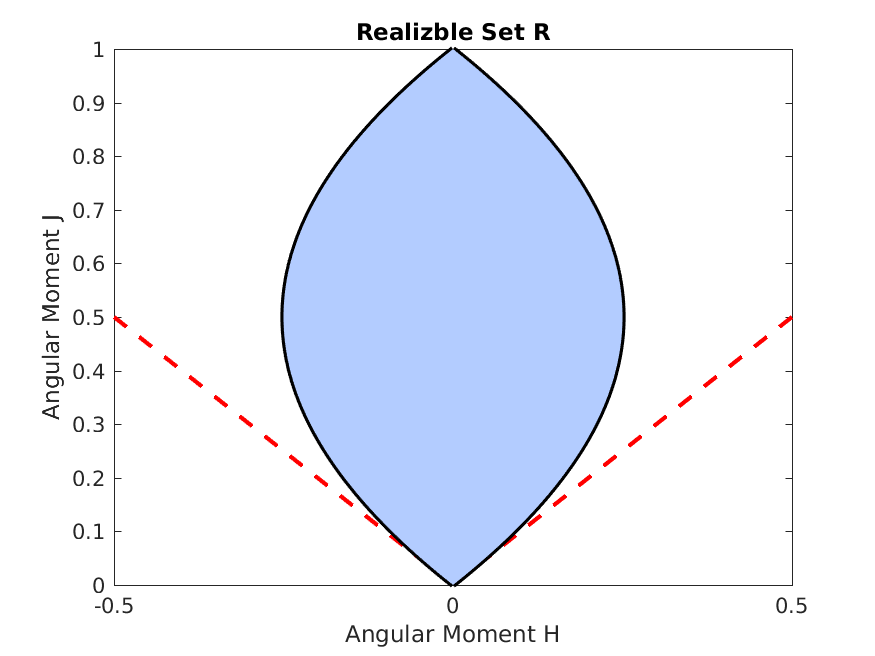
\includegraphics[width=1.0\linewidth]{figures/RealizableSetFermionic}
  \caption{Illustration of the realizable set $\cR$ defined in Eq.~\eqref{eq:realizableSet}.  
  The black lines define the boundary of $\cR$: $\gamma(\vect{\cM}) = 0$ while the dash red lines is the boundary given by the Maxwell's distributions.}
  \label{fig:RealizableSetFermionic}
\end{figure}

For the realizability-preserving scheme, we state some additional results.  
\begin{lemma}
  Let $\big\{\cJ_{a},\vect{\cH}_{a},\vect{\cK}_{a}\big\}$ be defined as in Eq.~\eqref{eq:angularMoments} with distribution function $f_{a}(\omegaNu)\in[0,1]\,\forall\,\omegaNu\in\bbS^{2}$.  
  Similarly, let $\big\{\cJ_{b},\vect{\cH}_{b},\vect{\cK}_{b}\big\}$ be moments of a distribution function $f_{b}\in[0,1]\,\forall\,\omegaNu\in\bbS^{2}$.  
  Let $\Phi^{\pm}(\vect{\cM})=\f{1}{2}\big(\vect{\cM}\pm\widehat{\vect{e}}\cdot\vect{\cF}(\vect{\cM})\big)$, where $\widehat{\vect{e}}\in\bbR^{3}$ is an arbitrary unit vector, and $\widehat{\vect{e}}\cdot\vect{\cF}(\vect{\cM})=\big(\widehat{\vect{e}}\cdot\vect{\cH},\widehat{\vect{e}}\cdot\vect{\cK}\big)^{T}$.  
  Then
  \begin{equation*}
    \vect{\cM}_{ab} = \big(\cJ_{ab},\vect{\cH}_{ab}\big)^{T} \equiv \Phi^{+}(\vect{\cM}_{a})+\Phi^{-}(\vect{\cM}_{b})\in\cR.
  \end{equation*}
  \label{lem:explicitStep}
\end{lemma}
\begin{proof}
  It is straightforward to rewrite the components of $\vect{\cM}_{ab}$ as
  \begin{equation*}
    \cJ_{ab}=\f{1}{4\pi}\int_{\bbS^{2}}f_{ab}(\omegaNu)\,d\omegaNu
    \quad\text{and}\quad
    \vect{\cH}_{ab}=\f{1}{4\pi}\int_{\bbS^{2}}f_{ab}(\omegaNu)\,\vect{\ell}(\omegaNu)\,d\omegaNu,
  \end{equation*}
  where $f_{ab}(\omegaNu)=\theta\,f_{a}(\omegaNu)+(1-\theta)\,f_{b}(\omegaNu)$ and $\theta(\omegaNu)=(1+\widehat{\vect{e}}\cdot\vect{\ell}(\omegaNu))/2\in[0,1]$.  
  Then, since $f_{ab}(\omegaNu)\in[0,1]\,\forall\,\omegaNu\in\bbS^{2}$, we have from Lemma~\ref{lem:MomentRealizable} that $\vect{\cM}_{ab}\in\cR$.  
\end{proof}

\begin{lemma}
  Let $\vect{\cM}_{a}=(\cJ_{a},\vect{\cH}_{a})^{T}\in\cR$ and $\alpha>0$.  
  Let $\vect{\cM}_{b}=(\cJ_{b},\vect{\cH}_{b})^{T}$ satisfy
  \begin{equation*}
    \vect{\cM}_{b}=\vect{\cM}_{a}+\alpha\,\vect{\cC}(\vect{\cM}_{b}), 
  \end{equation*}
  where $\vect{\cC}(\vect{\cM})=\vect{\eta}-\vect{\cD}\,\vect{\cM}$ is the collision term in Eq.~\eqref{eq:collisionTermMoments}.  
  Then $\vect{\cM}_{b}\in\cR$.  
  \label{lem:implicitStep}
\end{lemma}

\begin{proof}
  The first component of $\vect{\cM}_{b}$ can be written as
  \begin{equation}
    \cJ_{b}=\f{1}{4\pi}\int_{\bbS}f_{b}(\omegaNu)\,d\omegaNu,
  \end{equation}
  where $f_{b}(\omegaNu)=\theta\,f_{a}(\omegaNu)+(1-\theta)\,f_{0}$ and $\theta=1/(1+\alpha\,\xi)\in[0,1]$.  
  Then, since $f_{b}(\omegaNu)\in[0,1]\,\forall\,\omegaNu\in\bbS^{2}$, $\cJ_{b}\in[0,1]$.  
  Similarly, we can write
  \begin{equation*}
    \vect{\cH}_{b}=\f{(1+\alpha\,\xi)}{(1+\alpha)}\,\widetilde{\vect{\cH}}_{b},
    \quad\text{where}\quad
    \widetilde{\vect{\cH}}_{b}=\f{1}{4\pi}\int_{\bbS^{2}}f_{b}(\omegaNu)\,\vect{\ell}(\omegaNu)\,d\omegaNu.  
  \end{equation*}
  It follows from Lemma~\ref{lem:MomentRealizable} that $\widetilde{\vect{\bcM}}_{b}=(\cJ_{b},\widetilde{\vect{\cH}}_{b})^{T}\in\cR$.  
  Then, since $0\le\xi\le1$, we have $|\vect{\cH}_{b}|\le|\widetilde{\vect{\cH}}_{b}|\le(1-\cJ_{b})\,\cJ_{b}$.  
\end{proof}

\begin{lemma}
  Let $\vect{\cM}_{a}$ and $\alpha$ be given as in Lemma~\ref{lem:implicitStep}, and let $\vect{\cM}_{b}$ satisfy
  \begin{equation*}
    \vect{\cM}_{b}=\vect{\cM}_{a}+\alpha\,\vect{\cD}\,\vect{\cC}(\vect{\cM}_{b}),    
  \end{equation*}
  where $\vect{\cD}$ and $\vect{\cC}(\vect{\cM})$ are given by Eq.~\eqref{eq:collisionTermMoments},  then $\vect{\cM}_{b}\in\cR$.  
  \label{lem:correctionStep}
\end{lemma}
The proof follows along the same lines as the proof of Lemma~\ref{lem:implicitStep} and is omitted.  
